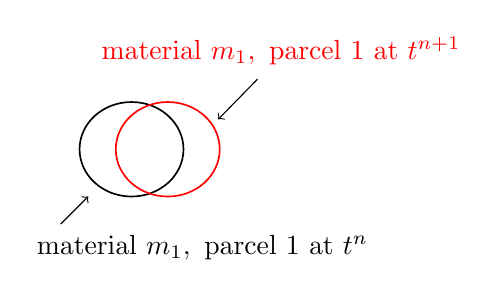
\begin{tikzpicture}
  \draw[semithick] (1.4,1.95) ellipse [x radius=0.66cm, y radius=0.6cm];
  \draw[semithick, red] (1.86,1.95) ellipse [x radius=0.66cm, y radius=0.6cm];

\node at (2.3,0.7){$\textcolor{black}{ \mbox{material } m_{1},\mbox{ parcel } 1 \mbox{ at } t^{n}}$};


\node at (3.3,3.2){$\textcolor{red}{ \mbox{material } m_{1},\mbox{ parcel } 1 \mbox{ at } t^{n+1}}$};





  \draw[->] (0.5,1) -- (0.85,1.35);
  \draw[->] (3,2.84) -- (2.5,2.33);
\end{tikzpicture}